\documentclass[12pt, %
openright, 
oneside, %
%twoside, %TCC: Se seu texto tem mais de 100 páginas, descomente esta linha e comente a anterior
a4paper,    %
%english,   %
brazil]{facom-ufu-abntex2}

\usepackage{graphicx}
\graphicspath{{figuras/}{pictures/}{images/}{./}} % where to search for the images

\newcommand{\blue}[1]{\textcolor{blue}{#1}}
\newcommand{\red}[1]{\textcolor{red}{#1}}


% ---
% Pacotes adicionados por mim (além dos do modelo!)
% ---
\usepackage[autostyle=true]{csquotes}   %Pacote de quotations (aspas)


% ---
% Informações de dados para CAPA e FOLHA DE ROSTO
% ---

\autor{Vinícius Henrique Almeida Praxedes} %TCC
\data{2023, Novembro}
\orientador{Daniel Duarte Abdala} %TCC
%\coorientador{Algum?} %TCC

\titulo{Paralelização de Algoritmos Notórios de Agrupamento de Dados em GPUs NVIDIA} %TCC

\hypersetup{pdfkeywords={palavra 1}{palavra 2}{palavra 4}{palavra 4}{palavra 5}} %TCC

% ? ############################################################################
% ? Variáveis e macros
% ? ############################################################################

\def\qntAlgrtm{dois}
\def\qntAlgrtmNaoExtenso{2}

% ? ############################################################################

\begin{document} 
\frenchspacing 

% ----------------------------------------------------------
% ELEMENTOS PRÉ-TEXTUAIS
% ----------------------------------------------------------
%\pretextual
\imprimircapa
\imprimirfolhaderosto


% ---
% Inserir folha de aprovação
% ---
%
% \includepdf{folhadeaprovacao_final.pdf} %TCC: depois de aprovado o trabalho, descomente esta linha e comente o próximo bloco para incluir scan da folha de aprovação.
%
\begin{folhadeaprovacao}

  \begin{center}
    {\ABNTEXchapterfont\large\imprimirautor}

    \vspace*{\fill}\vspace*{\fill}
    {\ABNTEXchapterfont\bfseries\Large\imprimirtitulo}
    \vspace*{\fill}
    
    \hspace{.45\textwidth}
    \begin{minipage}{.5\textwidth}
        \imprimirpreambulo
    \end{minipage}%
    \vspace*{\fill}
   \end{center}
    
   Trabalho aprovado. \imprimirlocal, 01 de novembro de 2016: %TCC:

   \assinatura{\textbf{\imprimirorientador} \\ Orientador}  
   \assinatura{\textbf{Professor}}% \\ Convidado 1} %TCC:
   \assinatura{\textbf{Professor}}% \\ Convidado 2} %TCC:
   %\assinatura{\textbf{Professor} \\ Convidado 3}
   %\assinatura{\textbf{Professor} \\ Convidado 4}
      
   \begin{center}
    \vspace*{0.5cm}
    {\large\imprimirlocal}
    \par
    {\large\imprimirdata}
    \vspace*{1cm}
  \end{center}
  
\end{folhadeaprovacao}
% ---


%%As seções dedicatória, agradecimento e epígrafe não são obrigatórias.
%%Só as mantenha se achar pertinente.

% ---
% Dedicatória
% ---
%\begin{dedicatoria}
%   \vspace*{\fill}
%   \centering
%   \noindent
%   \textit{Dedico a \lipsum[10]}  %TCC:
%   \vspace*{\fill}
%\end{dedicatoria}
% ---

% ---
% Agradecimentos
% ---
%\begin{agradecimentos}
%Agradeço a \lipsum[30]. %TCC:
%\end{agradecimentos}
% ---

% ---
% Epígrafe
% ---
%\begin{epigrafe}
%    \vspace*{\fill}
%  \begin{flushright}
%    \textit{``Alguma citação que ache conveniente? \lipsum[10]''} %TCC:
%  \end{flushright}
%\end{epigrafe}
% ---



\begin{resumo} %TCC:
 % ! MUDAR ISTO!!!
 Segundo a \citeonline[3.1-3.2]{NBR6028:2003}, o resumo deve ressaltar o
 objetivo, o método, os resultados e as conclusões do documento. A ordem e a extensão
 destes itens dependem do tipo de resumo (informativo ou indicativo) e do
 tratamento que cada item recebe no documento original. O resumo deve ser
 precedido da referência do documento, com exceção do resumo inserido no
 próprio documento. (\ldots) As palavras-chave devem figurar logo abaixo do
 resumo, antecedidas da expressão Palavras-chave:, separadas entre si por
 ponto e finalizadas também por ponto.

 \vspace{\onelineskip}
    
 \noindent
 \textbf{Palavras-chave}: Até, cinco, palavras-chave, separadas, por, vírgulas. %TCC:
\end{resumo}

% ---
% inserir lista de ilustrações
% ---
\pdfbookmark[0]{\listfigurename}{lof}
\listoffigures*
\cleardoublepage
% ---

% ---
% inserir lista de tabelas
% ---
\pdfbookmark[0]{\listtablename}{lot}
\listoftables*
\cleardoublepage
% ---



% ---
% inserir lista de abreviaturas e siglas
% ---
\begin{siglas} %TCC:
  % \item[Fig.] Area of the $i^{th}$ component
  % \item[456] Isto é um número
  % \item[123] Isto é outro número
  % \item[Zézão] este é o meu nome
  \item[CPU] \textit{Central Processing Unit} --- Unidade de Processamento Central. O principal e mais importante processador num computador. CPUs modernas possuem capacidade razoável de processamento paralelo, com dezenas de núcleos
  \item[GPU] \textit{Graphics Processing Unit} --- Unidade de Processamento de Gráficos. Um coprocessador especializado para operações vetoriais, comumente usado para operações da computação gráfica, como renderização de imagens. GPUs modernas possuem capacidade altíssima de processamento paralelo, com centenas a milhares de núcleos
  \item[VRAM] \textit{Video Random Access Memory} --- Memória de Vídeo de Acesso Randômico. Um componente das GPUs que equivale à RAM das CPUs. Uma memória volátil de alta velocidade, usada para armazenamento de dados necessários às operações gráficas realizadas pela GPU
  \item[CUDA] [inserir informação]
\end{siglas}
% ---

%% ---
%% inserir lista de símbolos, se for adequado ao trabalho. %TCC:
%% ---
%\begin{simbolos}
%  \item[$ \Gamma $] Letra grega Gama
%  \item[$ \Lambda $] Lambda
%  \item[$ \zeta $] Letra grega minúscula zeta
%  \item[$ \in $] Pertence
%\end{simbolos}
%% ---

% ---
% inserir o sumario
% ---
\pdfbookmark[0]{\contentsname}{toc}
\tableofcontents*
\cleardoublepage
% ---





% ----------------------------------------------------------
% ELEMENTOS TEXTUAIS
% ----------------------------------------------------------
\textual

% * ############################################################################
\chapter{Introdução}
% * ############################################################################

A busca pelo menor tempo de execução é uma diretriz ubíqua na computação. Desde os primórdios da área buscamos algoritmos e procedimentos que, dados os mesmos parâmetros de entrada, executem a mesma tarefa na menor quantidade de tempo possível. Outros recursos como espaço de memória utilizado, eficiência energética ou uso da rede em muitos cenários são mais importantes que o tempo de execução, mas ainda assim ela continua sendo um dos mais estudados parâmetros para categorização e avaliação de algoritmos e procedimentos na computação. De fato o tempo de execução --- em ciclos, ou passos, de processamento --- é a métrica utilizada na análise de uma das maiores incógnitas da computação, o problema P versus NP.

% TODO
% TODO
% TODO: Adicionar no parágrafo acima uma citação básica sobre o problema P vs NP
% TODO
% TODO

Um grande avanço na quantidade de poder de processamento dos computadores e, portanto, diminuição do tempo de execução de algoritmos, foi a criação dos processadores multinúcleo, permitindo a paralelização de processos. A habilidade de poder executar duas ou mais ações simultaneamente possibilitou muitos ganhos palpáveis na velocidade de execução de algoritmos e procedimentos, porém introduziu uma necessidade de mudança na forma de se pensar em resoluções de problemas computacionalmente: paralelizar um algoritmo serial (não-paralelo) não é uma tarefa trivial, e requer cuidados especiais com concorrência no acesso a recursos da máquina, interdependência de dados e cálculos, sincronização, entre outros dilemas.

% TODO
% TODO
% ? TODO: Seria mais adequado o uso do termo "sequencial" ao invés de "serial", ao descrever algoritmos não-paralelos? Pesquisar isso!
% TODO
% TODO

Um dos componentes que mais utilizam da paralelização num computador moderno são as GPUs --- unidades de processamento gráfico, ou placas de vídeo --- que são basicamente processadores especializados em operações vetoriais, altamente paralelizadas, usualmente utilizadas para computação gráfica, e com sua própria memória dedicada, a VRAM. Enquanto processadores de uso geral, CPUs, costumam ter no máximo dezenas de núcleos para processamento paralelo, GPUs possuem dezenas, milhares, de núcleos para operações vetoriais.

No entanto, cada vez mais está sendo descoberto e aproveitado o potencial de uso das GPUs em atividades não apenas voltadas para renderização, interfaces e outras operações gráficas, mas sim para a computação de propósito geral. Diversos algoritmos modernos e antigos beneficiam-se imensamente do poder de alta paralelização proporcionado pelas GPUs, e com ferramentas como a biblioteca e linguagem CUDA criada pela NVIDIA, está cada vez mais fácil implementar o uso de placas de vídeo em conjunto com processadores convencionais nos mais variados algoritmos.

Nem todo algoritmo pode ser paralelizado, no entanto. Existem procedimentos e algoritmos que são inerentemente seriais (também chamados de sequenciais), como o cálculo do $n$-ésimo número da sequência de \textit{Fibonacci}, que requer que dois números prévios da sequência tenham sido calculados para obtermos o atual --- salvo, é claro, alguma descoberta teórica matemática do comportamento da sequência que nos permitisse uma nova maneira de calcular o $n$-ésimo elemento sem essa necessidade.

É importante entender também que nenhum algoritmo é paralelizável por completo. Sempre existirão partes de algoritmos que necessariametne devem ser executadas serialmente para seu funcionamento correto. Há um limite teórico de ganho máximo que pode ser obtido ao se paralelizar um algoritmo qualquer. Esse limite é definido pela Lei de Amdahl \cite{Amdahl-Law}: $\frac{1}{1-p}$, onde $p$ é a razão entre tempo de execução gasto rodando código paralelizável e tempo de execução gasto no total.

% TODO
% TODO
% ? TODO: Falar aqui também da Lei de Gustafson? Apresentada no artigo de 1988: Reevaluating Amdahl's Law. Pode ser bem importante! É uma estimativa menos pessimista que a Lei de Amdahl, que leva em conta o fato de que, ao se aumentar os recursos computacionais, geralmente os algoritmos passam a ser utilizados em datasets cada vez maiores, aumentando muito a parcela de tempo de execução gasta em código paralelo, enquanto a gasta em código serial se mantém praticamente constante
% TODO
% TODO

E é a paralelização de uma classe de algoritmos em particular que é o foco desta pesquisa: os algoritmos de agrupamento de dados, também chamados de clusterização de dados, ou de \textit{clustering}. Tais algoritmos, de forma sucinta, agrupam objetos de maneira que os objetos no mesmo grupo, ou \textit{cluster}, sejam mais parecidos entre si, de acordo com alguma métrica, do que com objetos de outros grupos. A análise de clusters é essencial em diversas áreas da computação e estatística, como mineração de dados, aprendizado de máquina, compressão de dados, entre outras.

% TODO
% TODO
% ! TODO: Checar se essa citação abaixo, do site da NVIDIA, está correta! Esse bagulho no Bib usou o modelo "misc", não sei se está correto. O Mendeley gerou assim, então talvez esteja…
% TODO
% TODO

A hipótese principal deste trabalho é a de que algoritmos de clustering, em geral, são altamente paralelizáveis e apresentam um ganho considerável de desempenho (menor tempo de execução) quando implementados para utilizar o poder de paralelismo vetorial de placas de vídeo NVIDIA, através da linguagem CUDA \cite{CUDAZone}. Mais que isso, através de uma análise sistemática de estudos prévios e implementações de tais algoritmos em CUDA, visa-se generalizar o processo de paralelização destes. Isto é, identificar quais partes são necessariamente seriais, quais são paralelizáveis, e que sequência de passos gerais deve ser seguida para se conseguir paralelizar com sucesso um algoritmo de clustering qualquer e obter ganhos significativos de desempenho.

% TODO
% TODO
% ! TODO: Tenho que substituir essas referências abaixo por referências de versões seriais de cada algoritmo. Usar as referências das versões aceleradas em GPUs mais adiante, ao invés de aqui parece fazer bem mais sentido
% ! TODO: Adicionar o 
% TODO
% TODO

O foco de pesquisa são \qntAlgrtm{} algoritmos de agrupamento especialmente notórios: o \textit{K-means} \cite{GPU-accelerated-K-Means} e o \textit{Agrupamento Hierárquico}. Implementações e estudos realizados sobre estes foram analisados, e implementações paralelas em GPU tiveram seu desempenho comparado com as seriais em CPU.

% * Texto antigo do parágrafo acima:
% , \textit{DBSCAN} \cite{G-DBSCAN}, ou \textit{Clusterização Espacial Baseada em Densidade de Aplicações com Ruído}, e \textit{Random Forests} --- que mesmo não sendo exclusivamente um algoritmo de clusterização, pode ser utilizado justamente para tal.



% * ####################################

\section{Objetivos}



% * ####################################

\subsection{Objetivo Geral}

Este trabalho tem como objetivo principal testar a validez de sua hipótese (discutida mais à fundo na seção 1.2) de que algoritmos de clusterização são intrinsecamente paralelizáveis, e que o ganho de velocidade ao serem paralelizados é altamente significativo.

Além disso, deseja-se compilar aqui um vasto conhecimento de como paralelizar esses algoritmos em geral, analisando principalmente os \qntAlgrtm{} aqui estudados a fundo (K-Means e Agrupamento Hierárquico) e usando este aprendizado para criar um passo-a-passo genérico de como realizar tal modificação de código em um algoritmo de agrupamento qualquer.



% * ####################################

\subsection{Objetivos Específicos}

Para atingir o objetivo geral, é necessário completar diversos objetivos menores, ou \textit{milestones}, antes, criando um caminho de pesquisa que foi seguido --- não necessariamente na ordem apresentada. São estes:

\begin{itemize}
  \item Pesquisar extensamente a bibliografia da área, realizando assim um levantamento do estado da arte de algoritmos paralelos de agrupamento;
  
  \item Estudar implementações já realizadas dos \qntAlgrtm{} algoritmos aqui estudados, a fim de adquirir conhecimento de como a paralelização em CUDA deve ser realizada;
  
  \item Paralelizar um algoritmo de clustering \enquote{novo}, isto é, nunca antes paralelizado e exibido em trabalho científico, a fim de solidificar o conhecimento e prática de programação em CUDA. Foi escolhido o algoritmo de Agrupamento Hierárquico para tal;
  
  \item Quantificar o ganho de desempenho das implementações paralelas, realizando diversos experimentos de \textit{speedup}, usando diversos datasets de tamanhos e dimensionalidades variadas;
  
  \item Comparar o código serial (sem paralelização) com o código paralelo dos \qntAlgrtm{} algoritmos analisados, extraindo assim um conhecimento de como paralelizar um algoritmo de clusterização genérico;
\end{itemize}



% * ####################################

\section{Hipótese}

A hipótese que esta pesquisa procura testar é a de que algoritmos de clusterização em geral são inerentemente vetoriais e, consequentemente, se beneficiariam significativamente de arquiteturas de processamento vetoriais, como uma unidade de processamento gráfico, ou GPU.

Um problema ser vetorial diz respeito ao escopo de tipos de dados relevantes ao problema. Grande parte dos problemas da computação são escalares, o que significa que eles lidam com dados unitários, como por exemplo \textit{integers} ou \textit{floats}, um de cada vez. Já um problema vetorial lida com dados que são conjuntos unidimensionais, chamados vetores, que são formados por vários itens unitários de dados agrupados.

Um algoritmo que tente resolver um problema vetorial terá desempenho maior quando executado num processador vetorial, isto é, um processador que possui um conjunto de instruções capaz de manipular vetores. Apesar de um algoritmo de um problema vetorial ainda puder ser implementado e executado com sucesso num processador escalar, o desempenho será menor pois os dados vetoriais do problema terão que ter seus elementos processados um a um pelo processador, já que ele não trabalha com vetores propriamente ditos em seu conjunto de instruções.

Grande parte do ganho de desempenho supracitado vem do paralelismo proporcionado pelos processadores vetoriais, como GPUs, ao manipular conjuntos maiores de dados de uma só vez, e em vários núcleos simultaneamente. A natureza vetorial da GPU permite economizar traduções de endereço de memória e operações de obtenção (\textit{fetch}) e decodificação (\textit{decode}) de instruções, se comparado com o processamento escalar de uma CPU, pelo fato de se necessitar, na GPU, um número muito menor de instruções e endereços de memória quando os dados estão agrupados em vetores, que podem ser manipulados e usados em operações como se fossem, cada um, apenas um item de dados.

Este trabalho, então, visa demonstrar que algoritmos de agrupamento de dados, em geral, são intrinsecamente vetoriais. Isto é, qualquer algoritmo de clustering concebível será de natureza vetorial, pois estes analisam dados e tentam agrupá-los de acordo com algum grau de semelhança entre eles, análise esta que pode ser feita usando conjuntos dos itens de dados (vetores), ao invés de individualmente, mesmo que o \textit{dataset} inicial possua apenas dados de natureza escalar. Logo, qualquer algoritmo de agrupamento teria uma parcela do seu código que seria paralelizável e, assim, ganhariam desempenho significativo com uma execução numa GPU. Mais que isso, a parcela de tempo de execução do algoritmo gasta rodando código paralelo cresceria de acordo com o tamanho do conjunto de dados sendo analisado, garantindo ganhos ainda maiores.



% * ####################################

\section{Justificativa}

A pesquisa feita aqui pode ser de grande utilidade para a área da computação e ciência de dados, além de impulsionar a implementação de mais algoritmos paralelos de agrupamento de dados.

Com a compilação de conhecimento realizada aqui a intenção é facilitar pesquisas posteriores na área de paralelização de algoritmos de agrupamento e motivar com os experimentos de ganho de desempenho novas implementações paralelas de outros algoritmos desta classe, ilustrando o quão importante é o uso de processadores vetoriais como GPUs para tornar o uso de algumas destas abordagens de agrupamento realmente práticas.

Além disso, a apresentação nesse estudo de um procedimento genérico para paralelizar qualquer algoritmo de agrupamento será de extrema utilidade para qualquer desenvolvedor ou pesquisador que desejar implementar uma versão acelerada em GPU de um algoritmo do tipo, mesmo este sendo totalmente novo. No mínimo, a pesquisa servirá de ponto de partida para o entendimento e aprendizado de como realizar tal modificação no código do algoritmo, e renderá uma implementação real que serve de base para estudos e otimizações, até se obter eventualmente uma implementação digna para uso prático.





% * ############################################################################
\chapter{Fundamentação Teórica}
% * ############################################################################

Para compreender a pesquisa científica aqui realizada, é necessário primeiro entender o que são algoritmos de agrupamento, tanto de maneira geral quanto específica, explorando os fundamentos e funcionamento dos \qntAlgrtm{} algoritmos pesquisados. Veremos que a complexidade de tempo desses algoritmos tendem a ser inconvenientemente altas ($O(n\cdot\log{n})$, $O(n^2)$ ou até $O(n^3)$ sendo complexidades comuns) e por isso qualquer ganho de velocidade significativo obtido será de imensa relevância para a usabilidade prática do algoritmo.

Também é imprescindível explorar o funcionamento dos processadores vetoriais --- sendo as \textit{Unidades de Processamento Gráfico} (GPUs) o principal exemplo destes e exatamente no qual essa pesquisa irá focar --- e entender por que usá-los para paralelizar algoritmos de agrupamento proporcionará, em tese, um ganho de velocidade expressivo na execução destes, abrandando o peso de suas complexidades de tempo. Além de tudo isso, será apresentada brevemente a arquitetura utilizada para paralelizar os algoritmos estudados: a plataforma e modelo de programação CUDA, da NVIDIA, que permitirá extrair o poder de paralelização das placas de vídeo NVIDIA além de bibliotecas como a \textit{Numba}, que permite a programação vetorial facilitada na linguagem Python.



% * ####################################

\section{Agrupamento de dados}

% TODO #########################################################################
% TODO
% TODO: Continuar depois a revisão textual a partir deste comentário!
% TODO
% TODO #########################################################################

A clusterização, ou clustering, é a tarefa de agrupar um conjunto de elementos de modo que cada elemento de um grupo se \enquote{pareça} mais com outros elementos do grupo (cluster) que pertence do que com elementos dos grupos que não pertence --- para algum significado bem definido de semelhança. É um processo muito comum e virtualmente necessário nas áreas de mineração de dados, análise estatística, análise de imagem, aprendizado de máquina, reconhecimento de padrões, e muitas outras.

O significado de um cluster não pode ser bem definido e vai depender do conjunto de dados a ser analisado e a forma que os resultados obtidos serão utilizados --- de fato, esse é o principal motivo pelo qual tantos algoritmos diferentes de clustering existem \cite{SoManyClustAlg}. O comum em todas definições usadas é que um cluster é um conjunto de objetos de dados. Esses objetos são representados num espaço de dimensões iguais ao número de dados relevantes para cada objeto, e os algoritmos tentam criar grupos (clusters) nesse espaço que agrupem os objetos de uma maneira significativa, ou útil, para o estudo sendo feito e a definição de cluster sendo utilizada.

% TODO adicionar citações, figuras de agrumento de dados

% !!!!!!!!!!!!!!!!!!!!!!!!!!!!
% Talvez seria melhor colocar esse parágrafo num formato de lista? Não sei...
% Também não sei se meu uso do negrito aqui é permitido formalmente.
% !!!!!!!!!!!!!!!!!!!!!!!!!!!!

Diversos modelos de cluster podem ser usados para definir o que é um cluster: \textbf{modelos de centroide}, onde cada cluster possui um centro e os objetos pertencerão aos clusters com centros mais próximos deles, dada uma definição de distância no espaço de dados; \textbf{modelos de densidade}, que definem clusters como regiões densas e conexas no espaço de dados, contrastando com regiões menos densas que separam os clusters; \textbf{modelos de conectividade}, que constroem clusters a partir de conexões de objetos por distância; \textbf{modelos de distribuição}, que utilizam de distribuições estatísticas, como a distribuição normal ou exponencial, para modelar agrupamentos dos objetos; entre dezenas de outros modelos. Entender o modelo de cluster utilizado é essencial para compreender um algoritmo de clusterização e as diferenças entre a multitude destes.

% !!!!!!!!!!!!!!!!!!!!!!!!!!!!
% Eu preciso realmente ficar colocando termos em inglês não traduzidos (intraduzíveis de maneira sã, na maioria das vezes) em itálico? Isso me parece bem brega.
% !!!!!!!!!!!!!!!!!!!!!!!!!!!!

O resultado, ou saída, de um algoritmo de clusterização é comumente um rotulamento dos objetos de dados passados na entrada, o que indicará a divisão em clusters feita por ele. Classificações podem ser feitas quanto à natureza da clusterização obtida pelos algoritmos: \textbf{\textit{hard clustering}}, onde cada objeto pertence ou não a um cluster; \textbf{\textit{fuzzy clustering}}, onde cada objeto pertence uma certa porcentagem a cada cluster, o que pode significar, por exemplo, a chance do objeto pertencer àquele cluster \cite{FuzzyClusteringSurvey}. E subclassificações mais granulares ainda podem ser definidas, como: \textbf{clusterização de particionamento estrito}, onde cada objeto pertence a exatamente um cluster; \textbf{clusterização de particionamento estrito com \textit{outliers}}, onde objetos pertencem a exatamente um cluster, ou nenhum cluster, assim sendo considerados \textit{outliers}.



% * ####################################

\section{Programação Vetorial}

% ? ################
% ? Planning writing
% ? ################

[Escrever uma sub-seção sobre Programação Vetorial]

\begin{itemize}
  \item Tópico histórico, de onde ela vem, pra que ela serve
  \item Processadores que dão suporte pra operações vetoriais (hoje em dia, basicamente apenas GPUs. APUs tbm?)
  \item História da NVIDIA criando o CUDA
  \item Mudança de paradigma em relação à programação serial: escalar -> vetorial
\end{itemize}



% * ####################################

\section{NVIDIA CUDA}

[Escrever uma sub-seção sobre programação em CUDA]

\begin{itemize}
  \item O que é?
  \item Exemplos básicos de código  
  \item Como criar um projeto cuda, onde vai cada parte (sequencial, vetorial, etc)
\end{itemize}



% * ####################################

\section{Algoritmo 1: K-Means}

[Escrever uma sub-seção sobre o K-Means]

\begin{itemize}  
  \item Um dos algoritmos mais tradicionais, explicar a história dele
  \item Explicar Como ele é usado
\end{itemize}



% * ####################################

\section{Algoritmo 2: Hierarchical Clustering}

[Escrever uma sub-seção sobre o Hierarchical Clustering]





% * ############################################################################

% \chapter{Levantamento do Estado da Arte}

% ?
% ?
% ? Precisamos mesmo de um capítulo para isto? Talvez uma seção/sub-seção em algum outro capítulo/seção caiba melhor
% ?
% ?





% * ############################################################################
\chapter{Metodologia de Desenvolvimento e Pesquisa}
% * ############################################################################

% TODO
% TODO
% TODO Adicionar aqui uma figura, um diagrama, explicativo, sobre a metodologia usada para paralelizar um algoritmo de agrupamento genérico (vide arquivo ../Notes_230922_171133.pdf)
% TODO
% TODO

A pesquisa realizada neste trabalho consiste de estudos e análises de trabalhos prévios, desenvolvimento de uma versão paralelizada de um algoritmo de clustering e experimentos sobre essa implementação. Pode-se dividir tal metodologia em um conjunto de etapas.

A primeira etapa consiste de uma extensa pesquisa bibliográfica. O intuito é levantar o estado da arte na área de algoritmos de clusterização acelerados em GPU usando a linguagem e livraria CUDA da NVIDIA. Entender quais algoritmos já foram implementados com sucesso em CUDA, e como foi feita tal implementação, além dos resultados (ganhos em desempenho) das mesmas. Essa etapa agregará conhecimento sobre como utilizar CUDA para acelerar algoritmos de clustering, além de dar uma ideia do tipo de ganho de desempenho esperado de uma paralelização média desse tipo de algoritmo.

A segunda etapa consiste da implementação de uma versão paralela \enquote{inédita} de algum algum algoritmo de clusterização, ou seja, paralelizar um algoritmo nunca antes paralelizado e exibido em alguma pesquisa. Usando o aprendizado adquirido na primeira etapa de pesquisa, um algoritmo será paralelizado em CUDA, e seus resultados comparados com os resultados da versão serial (rodando somente numa CPU) para garantir corretude. Os ganhos de velocidade da versão acelerada em CUDA será então comparada também com os ganhos obtidos nos trabalhos analisados na primeira etapa. Isso servirá como uma medição da efetividade da implementação feita.

A terceira etapa consiste da busca de um procedimento geral para paralelizar um algoritmo de clustering genérico. Ou seja, encontrar um passo-a-passo de modificações ao código de um algoritmo serial que, ao fim, o transforme numa versão acelerada usando CUDA desse mesmo algoritmo, ainda mantendo sua corretude e proporcionando algum ganho de desempenho.

A quarta etapa, por fim, se trata de diversos experimentos de ganho de velocidade, ou \textit{speedup}, do algoritmo que teve aqui sua versão acelerada em GPU implementada e apresentada. Esses experimentos irão dar uma ideia do quão significativo foi o ganho de desempenho ao paralelizar o algoritmo usando CUDA, se há um teto ou chão para tais ganhos, como o \textit{speedup} aumenta ou diminui com o aumento do dataset a ser analisado, assim como realizar uma análise de outros parâmetros importantes que não sejam velocidade, como uso de memória --- afinal, as VRAMs das placas de vídeo são comumente mais limitadas em tamanho que as RAMs utilizadas pelas CPUs.

\chapter{Experimentos e Datasets}

\chapter{Resultados}

\chapter{Conclusões e Trabalhos Futuros}



% ----------------------------------------------------------
% Capítulo - Cronograma
% ----------------------------------------------------------

% \chapter{Cronograma}

% A tabela abaixo representa o cronograma de pesquisa e desenvolvimento deste trabalho. Cada célula da mesma representa uma semana de tempo (sete dias corridos), considerando cada mês como tendo exatamente quatro semanas. O período coberto vai de dezembro de 2019 à julho de 2020, data estimada de término da conclusão desta monografia.

% \begin{figure}[h]
%     \centering
%     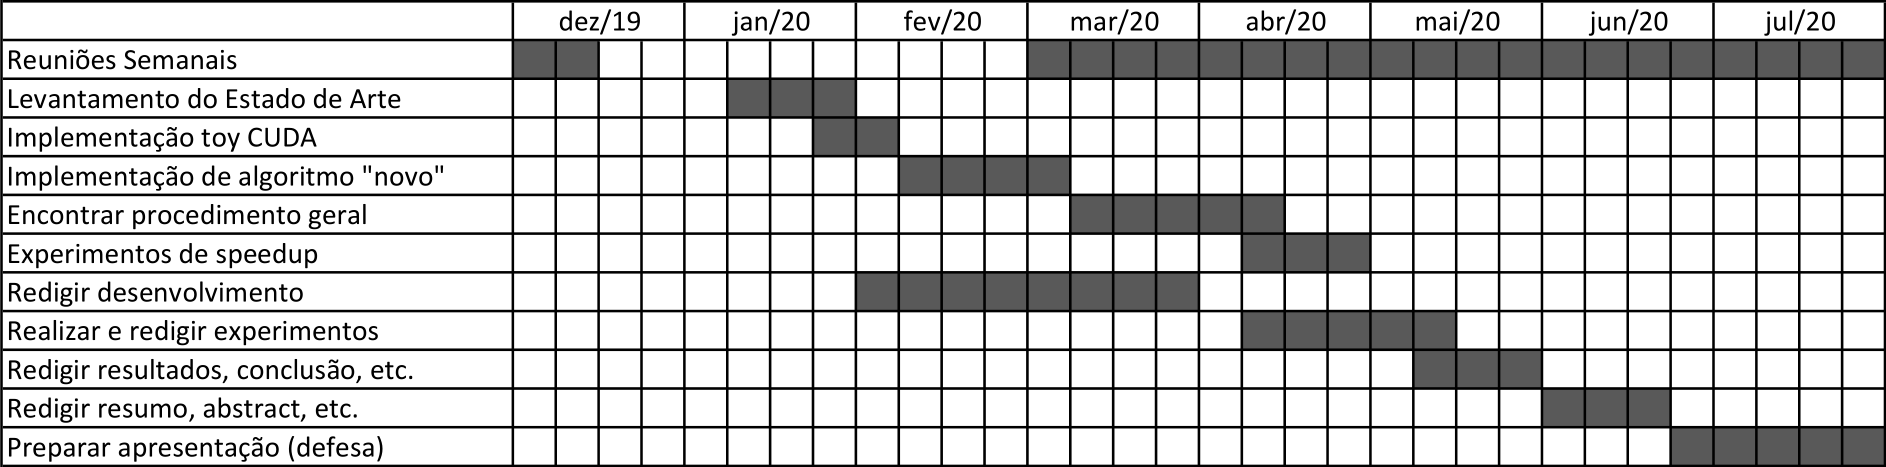
\includegraphics[width=\textwidth]{Cronograma_2-0}
%     \caption{Cronograma de pesquisa e desenvolvimento}
%     % \label{fig:my_label}
% \end{figure}


\chapter{Desenvolvimento}

\begin{figure}[!ht]
    \centering
  
\includegraphics[width=0.55\linewidth]{imagemExemplo.pdf}
  \caption[Isso é o que aparece no sumário]{Imagem de exemplo.}
  \label{fig:graficosVariandoTamanhoRede}
\end{figure}


%TCC:
%TCC:
%TCC:
%TCC:

% ---
% Conclusão
% ---
\chapter[Conclusão]{Conclusão}
%TCC:
E daí?





% ----------------------------------------------------------
% ELEMENTOS PÓS-TEXTUAIS
% ----------------------------------------------------------
\postextual


% ----------------------------------------------------------
% Referências bibliográficas
% ----------------------------------------------------------
\bibliography{references}


% %% ----------------------------------------------------------
% %% Apêndices TCC: só mantenha se for pertinente.
% %% ----------------------------------------------------------

% % ---
% % Inicia os apêndices
% % ---
% \begin{apendicesenv}

% % Imprime uma página indicando o início dos apêndices
% \part[apendices]{Apêndices}

% % ----------------------------------------------------------
% \chapter{Quisque libero justo}
% % ----------------------------------------------------------

% \lipsum[50]

% % ----------------------------------------------------------
% \chapter{Coisas que fiz e que achei interessante mas não tanto para entrar no corpo do texto}
% % ----------------------------------------------------------
% \lipsum[55-57]

% \end{apendicesenv}
% % ---


% ----------------------------------------------------------
% Anexos %TCC: so mantenha se pertinente.
% ----------------------------------------------------------

% ---
% Inicia os anexos
% ---
\begin{anexosenv}

% Imprime uma página indicando o início dos anexos
\part[anexos]{Anexos}

% ---
\chapter{Eu sempre quis aprender latim}
% ---

\lipsum[30]



% ---
\chapter{Coisas que eu não fiz mas que achei interessante o suficiente para colocar aqui}
% ---

\lipsum[31]



% ---
\chapter{Fusce facilisis lacinia dui}
% ---



\lipsum[32]

\end{anexosenv}

%---------------------------------------------------------------------
% INDICE REMISSIVO
%---------------------------------------------------------------------

\printindex



\end{document}